\subsubsection{MULTI-SCALE 3D INTERPRETATION}
The multi-scale is a technique to track objects that moves in 3 dimensions. 
To understand this technique we need to analyze the same object in 
two different positions, as in the Figure \ref{fig:multiscale3d}.

\begin{figure}[H]
\centering
  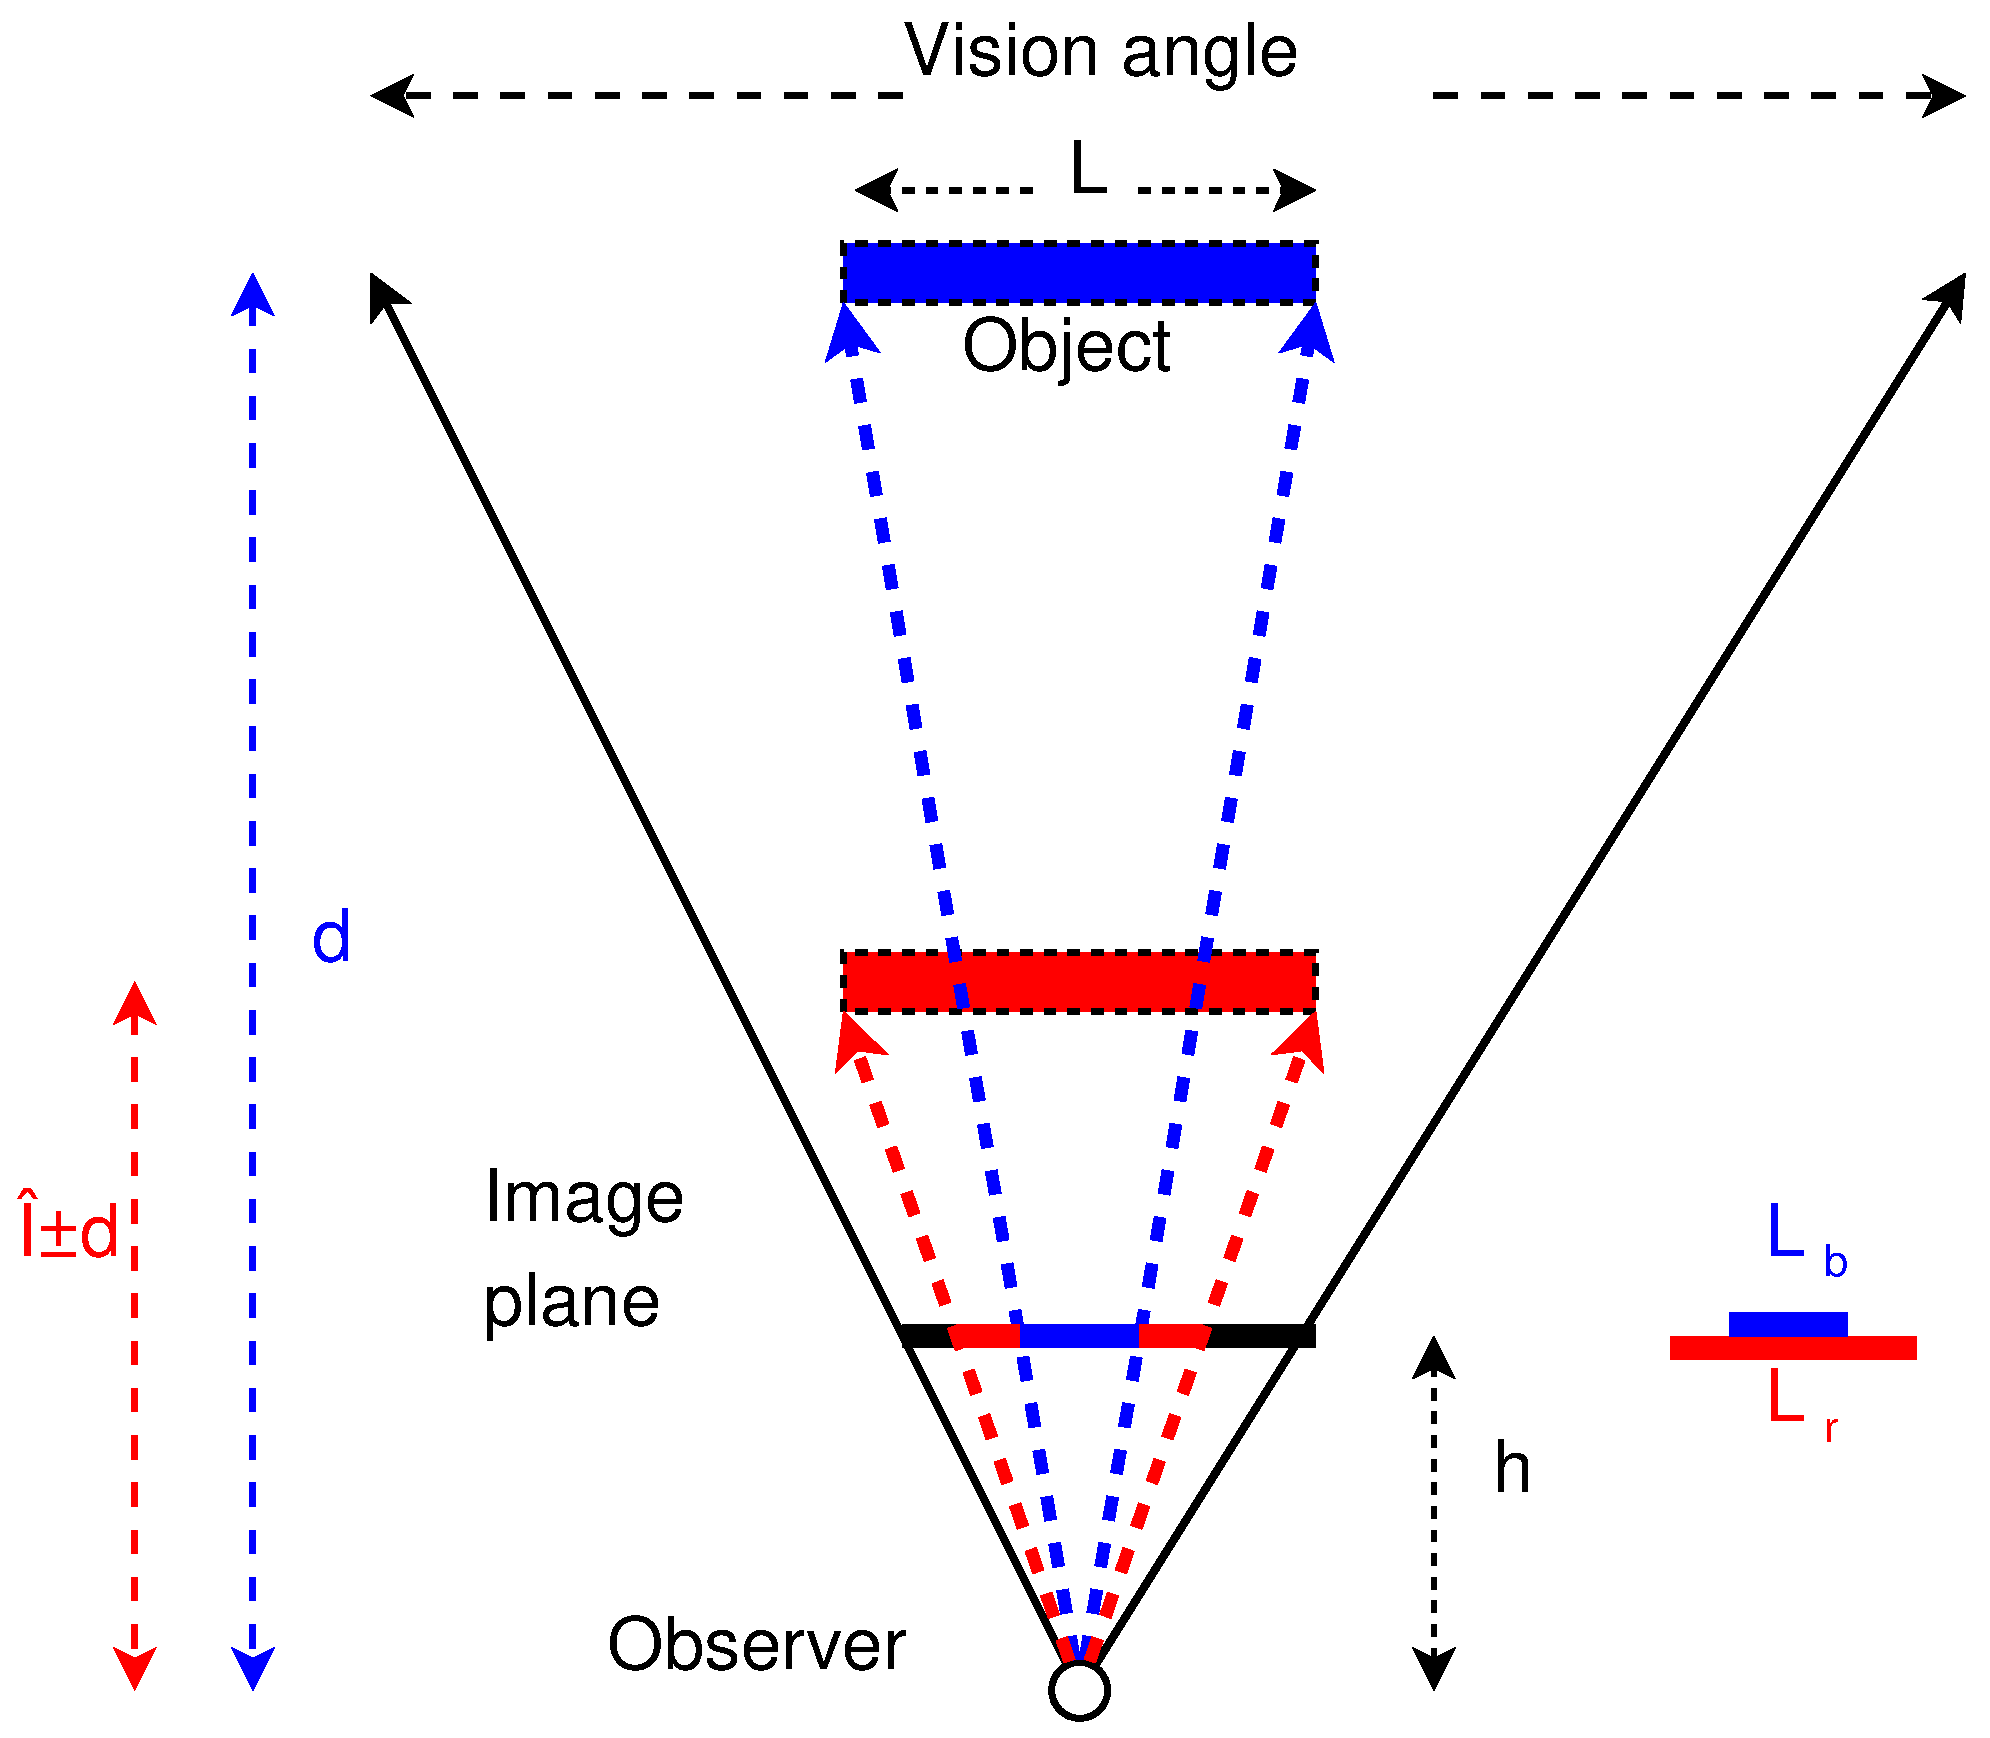
\includegraphics[width=.7\columnwidth]{images/Diagrama3.eps}
  \caption{Interpretation of the area relation in the multi-scale tracking.}
  \label{fig:multiscale3d}
\end{figure}
The figure show, using the colors blue and red, the same object located in two 
different distances, being these $d$ and $\alpha d$, respectively. 
In both cases, one picture of scene is obtained,
so that, the plane of photography is located at a distance $h$ of observer.
The projections of objects in blue and red, in plane of photography, are
called of $L_b$ and $L_r$, respectively.


The layers are organized of the smallest ($\alpha <1.0$) to the biggest ($\alpha >1.0$), 
to a set of discrete values of $\alpha$. 
With this proceeding, the algorithm is capable of track objects 
that in current frame are larger than in the last.

%usa Multi-resolution match criteria e explica isso dos tamanhos

\subsubsection{FACTOR OF APPROACHING - RELATIVE VELOCITY}
Factor of approaching is a dimensionless number related to the rate of approaching 
or departure of an object to the camera. The factor
is determined how showed at equation 2:

\begin{equation}
\centering
\everymath{\displaystyle}
f_a = \frac{Area_r}{Area_f} 
\end{equation}

Where $f_a$ is the factor of approaching, $Area_r$ is area of ROI and $Area_f$ 
is area of current frame.\\
The factor has two means, e.g., if the rate of approaching increase quickly, so 
the target is approaching. Or the apposite, if factor decreases, thus 
object is departing.\\
Relative velocity is calculate using a simples equation of kinematic in physics:


\begin{equation}
\centering
\everymath{\displaystyle}
 v = \frac{\Delta s}{\Delta t}
\end{equation}

Where $v$ is relative velocity, $\Delta s$ is difference in between two pixels and 
$\Delta t$ is time of proceeding.\\
Velocity calculated is relative for simple reason that it is impossible to know 
the real distance between the camera and object in this
condition.\\
